\documentclass[utf8]{beamer}

\usepackage{beamerthemesplit}
\usepackage{latexsym}
\usepackage{eurosym}
\usepackage[activeacute,spanish]{babel}
\usepackage{ae,aecompl}
\usepackage{graphicx}
\usepackage{amsfonts}


\mode<presentation>{
\usetheme{Warsaw}
\usecolortheme[RGB={148,20,110}]{structure}
\setbeamercovered{transparent}
}

\title{CONTROL DE GASTOS PERSONALES}
\subtitle {Proyecto del Primer Parcial}
\author{Vannesa Robles -  Ricardo Campuzano -  Ana Mora Ocaña}
\date{\today}
\institute {ESPOL}

\begin{document}
\begin{frame}[plain]{Lenguajes de programación}
\begin{center}

\includegraphics [width = 0.2 \textwidth]{logo.jpg} %para colocar el logo de la presentación
\end{center}
\titlepage
\end{frame}

%indice
\begin{frame}
\frametitle{Esquema} %Esquema es el titulo de la diapositiva
\tableofcontents[pausesections]
\end{frame}

\section{Problema a Resolver}
\begin{frame}[allowframebreaks]
\begin{block}{Problema a Resolver }
No hay un sistema de control de gastos personales de fácil uso, para las personas naturales (no obligadas a llevar contabilidad) , que deben declarar sus  impuestos en el SRI (Servicios de Rentas Internas). 
El proceso de llevar un control de sus actividades resulta dificultoso para las personas naturales ya que tienen que elaborar un informe de sus gastos e ingresos, para esto deben de recaudar previamente sus facturas, recordar fecha de declaración  y lo principal saber cómo hacerlo. 
Es este primordial interés, que nos vemos en la necesidad de digitalizar dicha información de una manera práctica; donde la persona podrá ahorrar tiempo y dinero porqué evitará archivar  papeletas de facturas y pagar multas por no recordar el día de su declaración,  además de tener una información actualizada de sus gastos.
\end {block}
\end{frame}


\section{Descripción de la Aplicación}
\begin{frame}[allowframebreaks]
\begin{block}{descripción de la aplicación}
Control de Gastos Personales es una aplicación en Android  diseñada para  personas naturales no obligadas a llevar contabilidad, que deben cumplir con la presentación de la información relativa a los gastos personales deducidos, por los constribuyentes, para efecto de liquidación de Impuesto a la Renta.
El objetivo de la aplicación  es desarrollar una herramienta que permita a los usuarios a llevar un mejor control de sus facturas. El usuario en el momento que haga una compra y tenga su factura en mano, podrá ingresar los datos de la factura e ir clasificando cada ingreso de datos en el tipo de gasto que corresponda.
La aplicación generará un reporte de gastos clasificados con la información ingresada de las facturas. Además dará la opción de descargarse dicho reporte, ayudará  recordando al usuario el día que le toque su declaración según el noveno digito de su cédula (Calendario Tributario), toda esta información de gastos lo mantendrá al día.
\end {block}
\end{frame}


\section{Aplicación}  
\begin{frame}[allowframbreaks]
\frametitle{Aplicación}
\begin{center}
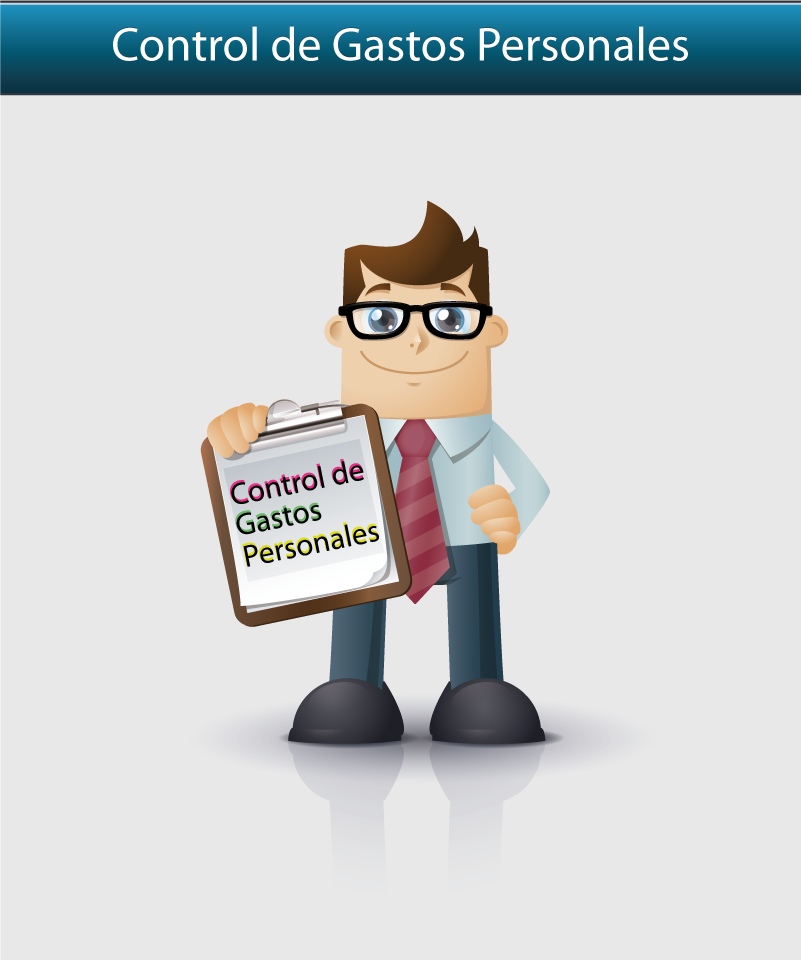
\includegraphics[width=0.3\textwidth]{cargando.png}
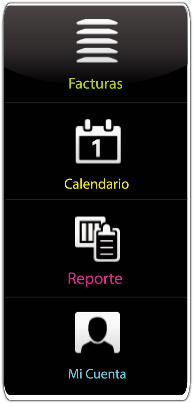
\includegraphics[width=0.3\textwidth]{menuprincipal.png}
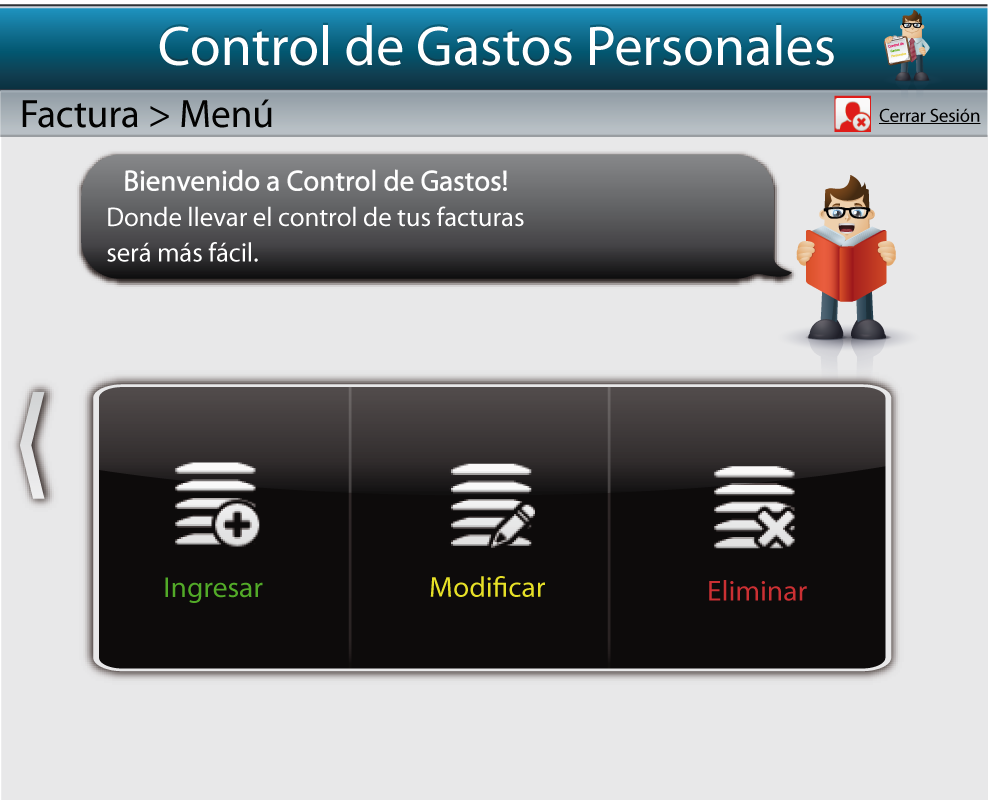
\includegraphics[width=0.3\textwidth]{factura.png}
\end{center}
\end{frame}

\begin{frame}[allowframbreaks]
\frametitle{Aplicación}
\begin{center}
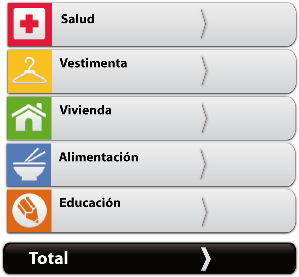
\includegraphics[width=0.3\textwidth]{informe_gastos.png}
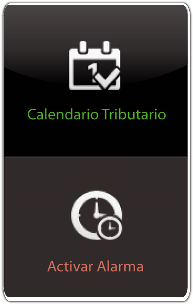
\includegraphics[width=0.3\textwidth]{alarma_over.png}
\end{center}
\end{frame}

\end{document}